\documentclass[border=3mm,tikz]{standalone}

\usepackage[utf8]{inputenc} 
% Preamble
	\usepackage{fullpage} % Package to use full page
	\usepackage{parskip} % Package to tweak paragraph skipping
	\usepackage{tikz} % Package for drawing
	\usepackage{amsmath}
	\usepackage{hyperref}
	\usepackage{amsmath,amssymb}
	\usepackage{color}
	\usepackage[version=4]{mhchem} 
	\usepackage{bm}
	\usepackage{verbatim}
	\usepackage{subfig}
	\usepackage{tkz-euclide}
	\usetkzobj{all}
	
	
	\usetikzlibrary{decorations.pathreplacing,angles,quotes}
	\usetikzlibrary{arrows,automata,positioning,backgrounds,calc,fadings}
	\usetikzlibrary{decorations.shapes}
	\usetikzlibrary{shapes,arrows,automata,positioning,fit,backgrounds,petri}
	\usetikzlibrary{fadings,decorations.pathmorphing}
	\usetikzlibrary{arrows,shapes}
%---------------------------start tikzstyle code --------------------------------------
	%---start green nodes---
		\tikzstyle{green} = [circle,thick, fill=green!70, scale=1,draw=black!30!green, font=\sffamily\large\bfseries] 
		\tikzstyle{green_orange} = [circle, thick, left color = green!80, right color=orange!70, scale=0.5,font=\sffamily\large\bfseries, shade border west to east=black!30!green to orange]  
		\tikzstyle{green_orange_reverse} = [circle, thick, left color = orange!70, right color = green!80,scale=0.32,font=\sffamily\large\bfseries, shade border west to 			east=orange to black!30!green]  
		\tikzstyle{green_blue} = [circle, thick, left color = green!90!black, right color = cyan!80, scale=1,font=\sffamily\large\bfseries,shade border west to east=black!30!green to blue]
		\tikzstyle{green_purple} = [circle,thick,left color = green!80, right color = violet!80, 	scale=0.32, font=\sffamily\large\bfseries, shade border west to east=black!30!green to 	violet]
	%---end green nodes---
	%---start blue nodes---
		\tikzstyle{blue} = [circle,thick,fill=cyan!80,scale=1,draw=blue!75!cyan,
		font=\sffamily\large\bfseries]
		\tikzstyle{blue_green} = [circle, thick, left color = blue!33!cyan, right color = cyan!50!yellow, scale=1,font=\sffamily\large\bfseries,shade border west to 			east=black!30!blue to green!70!black]
		\tikzstyle{blue_orange} = [circle,thick,left color = cyan, right color = orange!80, scale=1, font=\sffamily\large\bfseries, shade border west to east=blue to orange]
		\tikzstyle{blue_orange_reverse} = [circle,thick,left color = orange!80, right color = cyan, scale=1, font=\sffamily\large\bfseries, shade border west to east=orange to blue]
		\tikzstyle{blue_purple} = [circle,thick,left color = cyan!70!violet, right 				color = violet!80,scale=1, font=\sffamily\large\bfseries, shade border west to east=blue to violet]
		\tikzstyle{blue_red} = [circle,thick,left color = cyan, right color = magenta!80, scale=1, font=\sffamily\large\bfseries, shade border west to east=blue to magenta]
		\tikzstyle{blue_red_small} = [circle,thick,left color = cyan, right color = magenta!80, scale=1, font=\sffamily\large\bfseries, shade border west to east=blue to magenta]
	%---end blue nodes---
	%---start orange nodes---
		\tikzstyle{orange} = [circle,thick,fill=orange!55,scale=1,draw=orange, font=\sffamily\large\bfseries]
		\tikzstyle{orange_purple} = [circle,thick,left color = orange!70, right color = violet!80, scale=1, font =\sffamily\large\bfseries, shade border west to east=orange to violet]
		\tikzstyle{orange_yellow} = [circle,thick,left color = magenta!27, right color = yellow!80, scale=1, font =\sffamily\large\bfseries, shade border west to east=orange to yellow!75!orange]
	%---end orange nodes---
	%---start purple nodes---
		\tikzstyle{purple} = [circle,thick,fill=violet!45,scale=1,draw=violet!90, font=\sffamily\large\bfseries]
		\tikzstyle{purple_small} = [circle,thick,fill=violet!45,scale=1,draw=violet!90,
		font=\sffamily\large\bfseries]
		\tikzstyle{purple_orange} = [circle,thick,left color = violet!80, right color = orange!70, scale=1, font=\sffamily\large\bfseries, shade border west to east=violet to orange]
		\tikzstyle{purple_red} = [circle,thick,left color = violet!80, right color = magenta, scale=1, font=\sffamily\large\bfseries, shade border west to east=violet to orange]
		\tikzstyle{purple_blue} = [circle,thick,left color = violet!80, right 						color = cyan,scale=1, font=\sffamily\large\bfseries, shade border west to east=violet to blue]
	%---end purple nodes---
	%---start red nodes---
		\tikzstyle{red} = [circle,thick,fill=magenta!45,scale=1,draw=magenta!90,
		font=\sffamily\large\bfseries]  
		\tikzstyle{red_small} = [circle,thick,fill=magenta!45,scale=1,draw=magenta!90,
		font=\sffamily\large\bfseries] 
		\tikzstyle{red_blue} = [circle,thick,left color = magenta!80, right color = cyan, scale=1, font=\sffamily\large\bfseries, shade border west to east=magenta to blue]
		\tikzstyle{red_purple} = [circle,thick,left color = magenta!66, right color = violet!66, scale=1, font=\sffamily\large\bfseries, shade border west to east=magenta to violet]
	%---end red nodes---
	%---start miscellaneous nodes---
		%\tikzstype{square} = [square,thick,scale=0.1,draw]
		\tikzstyle{square}=[square,fill=white,minimum size=10pt,inner sep=0pt,scale=1]
		\tikzstyle{circle_dot}=[circle,fill=white,draw,node distance=3cm,norm/.style = [circle,fill=black,draw,minimum size=0.2cm] 
		\tikzstyle{vertex_large}=[circle,fill=white,minimum size=10pt,inner sep=0pt]
		\tikzstyle{vertex_small}=[circle,thick,draw=black,fill=white,minimum size=10pt,inner sep=0pt,scale=1]
		\tikzstyle{vertex}=[rectangle,fill=white,minimum size=10pt,inner sep=0pt]               
	%---end miscellaneous nodes-----
%--------------------------end tikzstyle code -------------------------			
%--------------------------start tikzstyle code -------------------------
	\definecolor{lavander}{cmyk}{0.33,0.66,0,0}
	\definecolor{violet}{cmyk}{0.79,0.88,0,0}
	\definecolor{burntorange}{cmyk}{0,0.52,1,0}	
	
	\def\lav{lavander!90}	
	\def\oran{orange!30}
		
	\tikzstyle{peers}=[draw,circle,violet,bottom color=\lav,
		top color= white, text=violet,minimum width=10pt]
	\tikzstyle{superpeers}=[draw,circle,burntorange, left color=\oran,
		text=violet,minimum width=20pt]
	\tikzstyle{legendsp}=[rectangle, draw, burntorange, rounded corners,
		thin,bottom color=\oran, top color=white,
		text=burntorange, minimum width=2.5cm]
	\tikzstyle{legendp}=[rectangle, draw, violet, rounded corners, thin,
		bottom color=\lav, top color= white,
		text= violet, minimum width= 2.5cm]
	\tikzstyle{legend_general}=[rectangle, rounded corners, thin,
		burntorange, fill= white, draw, text=violet,
		minimum width=2.5cm, minimum height=0.8cm]
	\tikzstyle{vertex}=[rectangle,fill=white,minimum size=10pt,inner sep=0pt]
%---------------------------end tikzstyle code --------------------------	
\makeatletter
\newif\iftikz@shading@path
\begin{document}
%-----------start Figure 1-------------
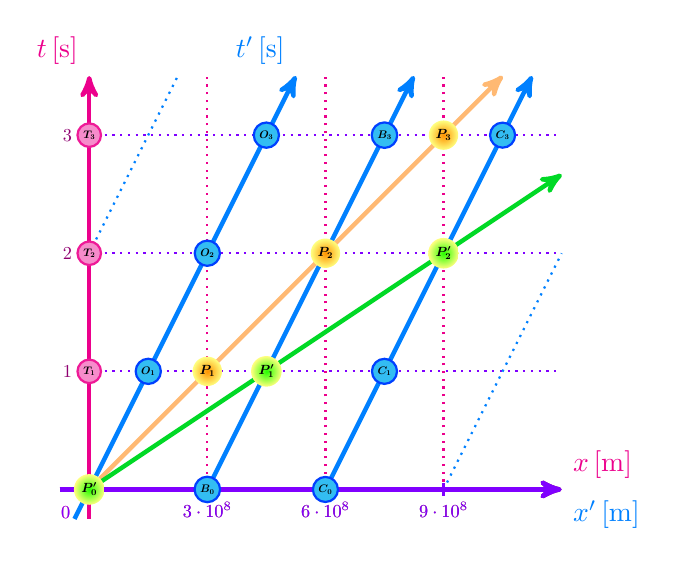
\begin{tikzpicture}[>=stealth',shorten >=0pt,auto,node distance=3cm,main node/.style={circle,thick, fill=white,scale=0.55,draw,font=\sffamily\large\bfseries},scale=1.5]
	%-----------start grid code ----------
		\def\figxmax{4};
		\def\figxmin{-0.25};
		\def\figymax{3.5};
		\def\figymin{-0.25};
		
		%\draw[step=0.5,very thin, black!15] (\figxmin,\figymin) grid (\figxmax,\figymax);
	%------------------end grid code --------------------
	%------------------start S frame grid code ------------
		\draw[thick,magenta,-,dotted] (1,0) -- (1,\figymax) node[anchor=south east] {};
		\draw[thick,magenta,-,dotted] (2,0) -- (2,\figymax) node[anchor=south east] {};
		\draw[thick,magenta,-,dotted] (3,0) -- (3,\figymax) node[anchor=south east] {};
		
		\draw[thick,blue!50!magenta,-,dotted] (0,1) -- (\figxmax,1) node[anchor=south east] {};
		\draw[thick,blue!50!magenta,-,dotted] (0,2) -- (\figxmax,2) node[anchor=south east] {};
		\draw[thick,blue!50!magenta,-,dotted] (0,3) -- (\figxmax,3) node[anchor=south east] {};
	%---------end S frame grid code --------------
	%--------------start S frame axes code ---------
		\def\xaxis{9};
		\foreach \x in {3,6,...,\xaxis} 
		\draw[thick,color=blue!25!purple] (\x cm /3, 1.5pt) -- (\x cm /3, -1.5pt) node[anchor=north, 	color=blue!25!purple,scale=0.66] {$\x \cdot 10^8$};
		\draw[ultra thick,blue!25!purple,->] (\figxmin,0) -- (\figxmax,0) node[anchor=south west,color=magenta] {$x \, [\mathrm{m}]$};
		
		\node(vertex) at (-0.2,-0.2) [color=magenta,scale=0.66]{0};
		
		\def\yaxis{3};
		\foreach \y in {1,...,\yaxis} 
		\draw[thick,color=magenta] (2pt,\y cm) -- (-2.5pt,\y cm) node[anchor=east, 			color=blue!25!purple, scale=0.66] {$\y$};
		\draw[ultra thick,magenta,->] (0,\figymin) -- (0,\figymax) node[anchor=south east] {$t \, [\mathrm{s}]$};             
	%--------end S frame axes code ------------
	%--------------------start S' frame grid code -----------------
		\draw[thick,blue!50!cyan,-,dotted] (0,2) -- (0.75,\figymax) node[anchor=south east] {};
		\draw[thick,blue!50!cyan,-,dotted] (1,0) -- (2.75,\figymax) node[anchor=south east] {};
		\draw[thick,blue!50!cyan,-,dotted] (2,0) -- (3.5,3) node[anchor=south east] {};
		\draw[thick,blue!50!cyan,-,dotted] (3,0) -- (4,2) node[anchor=south east] {};
	%-------end S' frame grid code -----------
	%---------start S' frame axes code ------------
		\def\xaxis{9};
		\foreach \x in {3,6,...,\xaxis} 
		\draw[thick,color=blue!50!magenta] (\x cm /3, 1.5pt) -- (\x cm /3, -1.5pt) node[anchor=north, color=blue!50!magenta,scale=0.66] {$\x \cdot 10^8$};
		
		\draw[color=blue!50!magenta,->,ultra thick] (\figxmin,0) -- (\figxmax,0) node[anchor=north west,color=blue!50!cyan] {$x' \, [\mathrm{m}]$};
		
		\node(vertex) at (-0.2,-0.2) [color=blue!50!magenta,scale=0.66]{0};
		
		\draw[ultra thick,blue!50!cyan,->] (-0.125,-0.25) -- (1.75,\figymax) node[anchor=south east] {$t' \, [\mathrm{s}]$};  
	%--end S' frame axes code ------
	%------tart T position nodes -------
		\coordinate (T0) at (0,0);
		\coordinate (T1) at (0,1);
		\coordinate (T2) at (0,2);
		\coordinate (T3) at (0,3);
		
		\node[red,scale=0.33] (T0) at (T0) {\textcolor{black}{\bm{$T_0$}}}; 
		\node[red,scale=0.33] (T1) at (T1) {\textcolor{black}{\bm{$T_1$}}}; 
		\node[red,scale=0.33] (T2) at (T2) {\textcolor{black}{\bm{$T_2$}}}; 
		\node[red,scale=0.33] (T3) at (T3) {\textcolor{black}{\bm{$T_3$}}}; 
	%-------------end T position nodes -------
	%-------------start O position nodes -----
		\coordinate (O0) at (0,0);
		\coordinate (O1) at (0.5,1);
		\coordinate (O2) at (1,2);
		\coordinate (O3) at (1.5,3);
		
		\node[blue,scale=0.33] (O0) at (O0) {\textcolor{black}{\bm{$O_0$}}};  
		\node[blue,scale=0.33] (O1) at (O1) {\textcolor{black}{\bm{$O_1$}}}; 
		\node[blue,scale=0.33] (O2) at (O2) {\textcolor{black}{\bm{$O_2$}}}; 
		\node[blue,scale=0.33] (O3) at (O3) {\textcolor{black}{\bm{$O_3$}}}; 
	%------end O position nodes -------------------			
	%--------------start B path code -----------------
		\coordinate (B0) at (1,0);
		\coordinate (B1) at (1.5,1);
		\coordinate (B2) at (2,2);
		\coordinate (B3) at (2.5,3);
		
		\draw[ultra thick,blue!50!cyan,->] (B0) -- (2.75,3.5);
		
		\node[blue,scale=0.33] (B0) at (B0) {\textcolor{black}{\bm{$B_0$}}};  
		\node[blue,scale=0.33] (B1) at (B1) {\textcolor{black}{\bm{$B_1$}}};
		\node[blue,scale=0.33] (B2) at (B2) {\textcolor{black}{\bm{$B_2$}}}; 
		\node[blue,scale=0.33] (B3) at (B3) {\textcolor{black}{\bm{$B_3$}}}; 				
	%---------------end B path code ----------	
	%--------------start B path code -----------------
		\coordinate (C0) at (2,0);
		\coordinate (C1) at (2.5,1);
		\coordinate (C2) at (3,2);
		\coordinate (C3) at (3.5,3);
		
		\draw[ultra thick,blue!50!cyan,->] (C0) -- (3.75,3.5);
		
		\node[blue,scale=0.33] (C0) at (C0) {\textcolor{black}{\bm{$C_0$}}};  
		\node[blue,scale=0.33] (C1) at (C1) {\textcolor{black}{\bm{$C_1$}}};
		\node[blue,scale=0.33] (C2) at (C2) {\textcolor{black}{\bm{$C_2$}}}; 
		\node[blue,scale=0.33] (C3) at (C3) {\textcolor{black}{\bm{$C_3$}}}; 				
	%---------------end B path code ----------
	%--------------start photon 1 path code -----------------
		\coordinate (P0) at (0,0);
		\coordinate (P1) at (1,1);
		\coordinate (P2) at (2,2);
		\coordinate (P3) at (3,3);
		
		\draw[ultra thick,orange!55,->] (P0) -- (3.5,3.5);
		
		\node[circle,thick,inner color = yellow!15!orange, outer color = yellow!50,scale=1, font=\sffamily\large\bfseries,scale=0.4] (P0) at (P0) {\textcolor{black}{\bm{$P_0$}}};  
		\node[circle,thick,inner color = yellow!15!orange, outer color = yellow!50,scale=1, font=\sffamily\large\bfseries,scale=0.4] (P1) at (P1) {\textcolor{black}{\bm{$P_1$}}};
		\node[circle,thick,inner color = yellow!15!orange, outer color = yellow!50,scale=1, font=\sffamily\large\bfseries,scale=0.4] (P2) at (P2) {\textcolor{black}{\bm{$P_2$}}}; 
		\node[circle,thick,inner color = yellow!15!orange, outer color = yellow!50,scale=1, font=\sffamily\large\bfseries,scale=0.4] (P3) at (P3) {\textcolor{black}{\bm{$P_3$}}}; 				
	%---------------end photon 1 path code ----------
	%--------------start photon 2 path code -----------------
		\coordinate (P0) at (0,0);
		\coordinate (P1) at (1.5,1);
		\coordinate (P2) at (3,2);
		
		\draw[ultra thick,blue!15!green,->] (P0) -- (4,2.6667);
		
		\node[circle,thick,inner color = yellow!15!green, outer color = yellow!50,scale=1, font=\sffamily\large\bfseries,scale=0.4] (P0) at (P0) {\textcolor{black}{\bm{$P'_0$}}};  
		\node[circle,thick,inner color = yellow!15!green,outer color = yellow!50,scale=1, font=\sffamily\large\bfseries,scale=0.4] (P1) at (P1) {\textcolor{black}{\bm{$P'_1$}}};
		\node[circle,thick,inner color = yellow!15!green, outer color = yellow!50,scale=1, font=\sffamily\large\bfseries,scale=0.4] (P2) at (P2) {\textcolor{black}{\bm{$P'_2$}}};  				
	%---------------end photon 2 path code ----------
\end{tikzpicture}
%--------------end Figure 1------------
\end{document}
